\chapter{Link Resource Tree Aggregation for Hierarchical Networks}
\label{chap:HierarchyRTAggregation}
\markright{Link Resource Tree Aggregation for Hierarchical Networks}

%======================================================================
\section{Introduction}
%======================================================================
As described in Chapter~\ref{cha:HierarchyOfNetworks}, transport networks consist of hierarchies of network switching layers as well as physically or logically divided domains. To achieve scalability in routing and network state advertisements, domains and switching layers advertise summary, or aggregated views of their internal structure to their peer and client layers. In other cases, topology aggregation is also needed for security reasons to hide the details of the underlying domain from others. In these cases, the aggregation scheme should not misrepresent information about the domains or layer's internal structure.

While Topology Aggregation (TA) is needed to ensure the scalability of the path selection schemes, the reliance on aggregate information to determine an appropriate path for a LSP connection request may sometimes result in infeasible paths being used-- ultimately leading to failing the call admission test at some intermediate intra-domain node. This type of a blockage (due to a discrepancy between actual and advertised information, or due to changes that might have occurred since the last advertisement) causes the LSP connection request to retrace its steps from the point of blockage back to its original entry point into the domain (\eg ABR node)-- a process described in previous chapter as a crankback. Once the request has returned to the point where it first entered the domain or layer, a new path through the domain can be computed; if such a path is found the LSP connection is established, otherwise the request cranks back further upwards towards its origin as shown in Figure~\ref{fig:crankback}. Crank-backs continue until either the network decides that no new path can be found, or the signaling protocol timers expire. Ultimately, the target in general when designing efficient resource and topology aggregation schemes is to have lower such frequency of crankbacks at signaling time which inherently indicates faster setup times for connections and less control traffic load.

\begin{figure}[t]
\centering
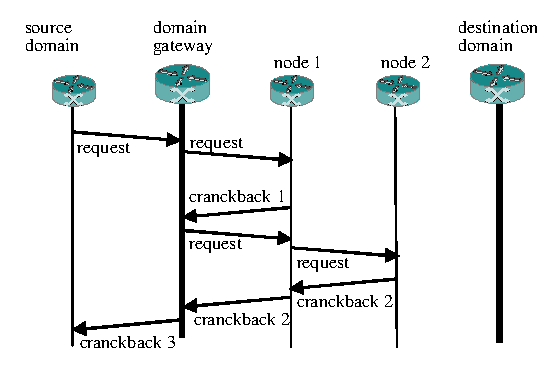
\includegraphics{Figures/crankback.eps}
\caption{Crankbacks with inter-domain signaling}
\label{fig:crankback}
\end{figure}

\section{Hierarchical Path Computation}
State-dependent QoS-enabled path computation schemes necessitate the provisioning of scalable routing solutions that take into account the QoS requirements of prospective LSP connections as well as the available network resources. Examples of such protocols are the Private Network-to-Network Interface (PNNI) and the QoS-enhanced OSPF protocol, both of which are link-state and inherently hierarchical.

In fact, no node in a real network holds the exact state of the complete network in real time due to inherent latencies in distributing the advertised link state parameters. Consequently, the chosen path at the source node may sometimes not guarantee the requested QoS, and each node along the signaled path has to perform its own call admission and that may end-up blocking the call. The goal of aggregation is to achieve a simplified representation of both topology and QoS advertisements.

Using a hierarchical path computation a path is computed based on a mixture of detailed and aggregated state information. A signaling or call-processing entity in each domain will compute intra-domain path or paths between border routers using detailed information about the domain's internal topology and advertises logical link state attributes to its neighboring domains-- see Figure~\ref{fig:TwoLevelHrchy}. Based on the aggregate advertisements between domains, the source-domain call processing entity or border node calculates a feasible inter-domain ``loose path'' for the connection that satisfies the end-to-end QoS requirement. As such, a hierarchical QoS network has to use a QoS aggregation scheme within each of its logical and corresponding physical layers.

\subsection{Topology and Link State Aggregation Procedure}
\label{TopologyLinkStateAggregation}
The extent of aggregation of information and what to aggregate play an important role in determining feasible paths and improving the chances of establishing an LSP request. Yet typically, very little information is conveyed to non-local lower level areas of the hierarchy, \eg in the previous example only prefix reachability information was provided by the BGP protocol. However, for some networks, this could cause significant problems when attempting to set up LSPs that guarantee bandwidth for traffic routed across multiple areas.

Alternatively, carriers can attempt to push a summary containing more information about their network link state to intra-level nodes. There is an important trade-off with doing that however-- \ie increasing the information included in the link state summary, will also increase the amount of information that needs to be stored, maintained, processed, and considered by intra-domain nodes in their path computation algorithms.

At one extreme, an aggregation scheme must not represent any information about a domain's internal structure. In this case, all possible aggregated representations that could be generated will have to include the costs of all possible transits through the domain. Such a representation may be viewed as a complete weighted graph whose vertices are the border nodes of the domain whose edges represent the costs of the corresponding transits. Unfortunately, the size of such a representation grows quadratically in the number of nodes, which implicates scalability problems.

The performance benefits of having higher-fidelity aggregation scheme need to be balanced against real-world burdens imposed by the use of larger representations. Such burdens include having grater space requirements for the topology database within each domain, increase background traffic between domains due to topology updates, and longer computation times for determining the least-cost paths.

The concept of levels is used to help aggregate properties of a particular area. One example of such aggregation would be to represent the Internet as a \emph{level-1} graph with vertices representing abstract nodes and edges representing the inter-domain links-- we refer to this as the simple-node representation. Another aggregation scheme would be to abstract the domain by its ABR that are connected by abstract links-- we refer to this as the complex-node representation. This can be viewed as a complete weighted graph whose vertices are the border nodes of the domain and whose edges represent the costs of the corresponding transits as shown in Figure~\ref{fig:TwoLevelHrchy}.

\begin{figure}[t]
\centering
\includegraphics[scale=0.75]{Figures/TwoLevelHrchy.eps}
\caption{Path computation in two level hierarchy networks}
\label{fig:TwoLevelHrchy}
\end{figure}

For example, consider the example of a 2-level hierarchical network in Figure~\ref{fig:TwoLevelHrchy}. In this example, the physical nodes and links are at the lowest level of the hierarchy. The higher level consists of abstract nodes and links that are summarization of the lower level topology.

Every node in each area discovers Link State information about the links and nodes inside that area. These links are physical links, and so they should be viewed as being part of the lowest level. At the higher level, each area is represented by an abstract node. If there is at least one physical link between two areas, then the corresponding abstract nodes have an abstract link between them. The set of abstract nodes at the higher level form a virtual area, and distribute information about each of the an abstract links amongst themselves.

Each abstract node ``feeds down'' summarized information about these abstract links to the lower level nodes in the area it represents. From the perspective of the lower level nodes, there is now a link between node A3 and area B.

It is important to note that the above aggregation scheme equally applies to horizontally adjacent domains at the same layer (\eg IP packet neighboring domains), as well as between vertically adjacent domains (\eg IP and optical layer domains). In the latter case, the border model scheme discussed in Chapter~\ref{cha:HierarchyOfNetworks}, can be used to flood logical link representations (also referred to as forwarding adjacencies) to higher layers (\eg packet layer). Consequently, these FA links can be used in the path computation for requests that are originate at packet layer.

\begin{figure}[t]
\centering
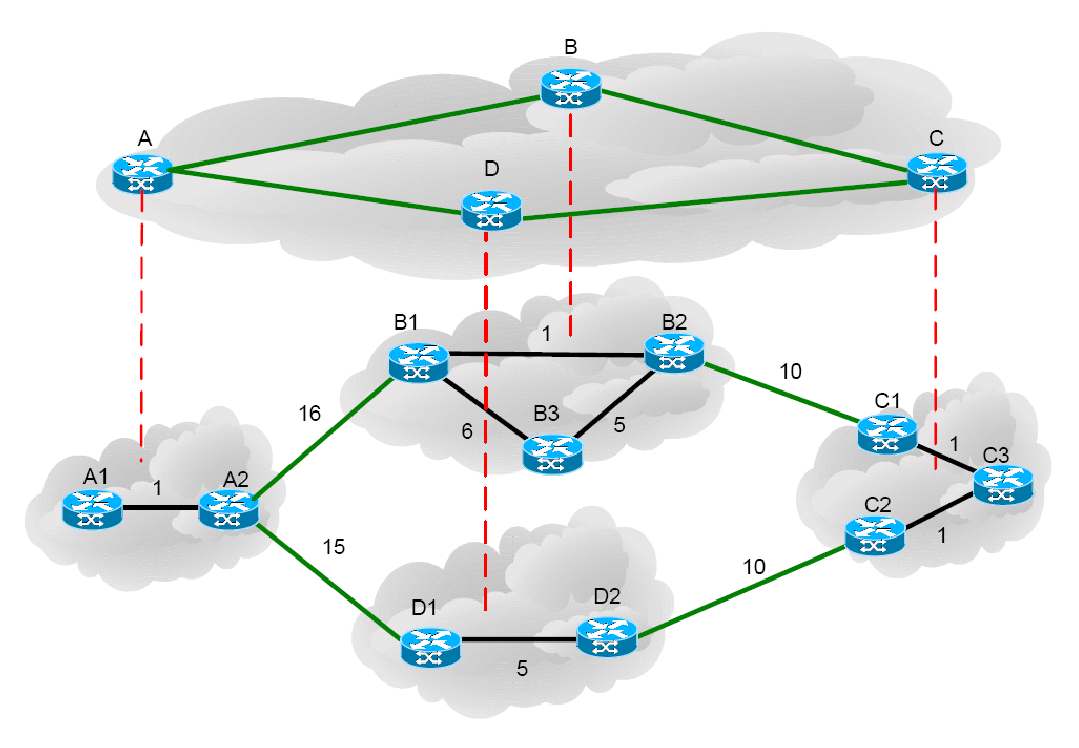
\includegraphics[scale=0.75]{Figures/TEVirtual.eps}
\caption{TE path computation with abstract links}
\label{fig:TEVirtual}
\end{figure}

\subsection{Simple and Complex Node Domain Abstraction}
Figure~\ref{fig:TEVirtual} provides an example of Simple Node Representation because each area is represented by a single node at the higher level of the hierarchy. However, this type of representation does not take into account differences in the Traffic Engineering constraints associated with different paths across an area.

In this case, determining the cost that should be associated with the logical links  (\eg link A-B) is problematic. If we do not include the cost of the intra-area links when calculating the cost of these logical links then it appears that the cost of A-B is 16 units, A-D is 15 and B-C and D-C are both 10. Given this, if A1 wanted to calculate a path to C3 it would select the path A1-A2-D-C. At the lower level, this path is actually A1-A2-D1-D2-C2-C3 which has a cost of 32 units, which might be unacceptable. Also, in this example, the path A1-A2-B1-B2-C1-C3, which was overlooked, costs just 29 units.

However, including the cost of the intra-area links is not straightforward. A carrier could configure a fixed cost to traverse each abstract node in any direction but this may not represent the lower level area topology. In the above example, if B1, B2 and B3 were all Area Edge Points, then the cost associated with traversing area B would be dependent on the direction in which the area is traversed. While B1 to B2 only has a cost of 1 unit, traversing the network from B1 to B3 costs at least 6 units.

Representing an entire area as an abstract node, these intra-area differences cannot be displayed in the routing protocol. To solve this problem, carriers may opt to use a different form of representation for each area-- the complex node representation.

Using the complex node representation, the underlying area is not advertised merely as a single abstract node-- but as a series of abstract nodes and links that illustrate, at the higher level, how the area can be traversed. Like any other links, these links can have properties such as available bandwidth, delay or cost associated with them. Exactly how a particular area is represented depends on the hierarchical routing protocol being used.

Suppose an abstract link is to be set up between A1 and A3 (the dotted line in Figure~\ref{fig:TEVirtual}). There are two possible paths across the area A1-A2-A3, A1-A4-A3. The first path between A1 and A3 has a greater amount of bandwidth available, the latter minimizes delay. In networks such as this, associating bandwidth values with the abstract link becomes difficult. If the larger available bandwidth (5000 Mbits/s) and the smaller end-to-end delay (10ms) are associated to the link it would appear, at the higher level, that the area is capable of supporting an LSP that requires 4000 Mbits/s and an end-to-end delay of 10ms. This is not true. However, if the carrier associates a lower bandwidth value with the abstract link (\eg 3000 Mbit/s) it appears, at the higher level, that the area cannot support LSPs that require 4000 Mbits/s of bandwidth at all, which again is untrue. To get round this problem, the area could be represented with multiple abstract links advertised between two nodes. However advertising more and more information into the higher level of hierarchy is not always desirable-- keeping in mind that the point of hierarchical routing is to minimize the amount of link state information that nodes in other areas/layers have to maintain.

\subsection{Limitations of Hierarchical Schemes}
Using the hierarchical model, setting up protected paths is still challenging job. For example in Figure~\ref{fig:TEVirtual}, assuming A1 is responsible for selecting the path , but that node is unaware of the intra-domain topology information needed to allow it to calculate a diverse path that could protect the original LSP. SRLG information could be associated to the abstract links for this reason. However meaningfully associating a set of SRLGs to an abstract node representing multiple areas may be very difficult.

In the next section, we present a novel scheme to aggregating SRLG information in the flooded logical links that will allow intra-domain link to compute diverse paths for their protected LSPs. 

\begin{figure}[t]
\centering
\includegraphics{Figures/LRT.eps}
\caption{Hierarchical link resource tree organization}
\label{fig:LRT}
\end{figure}

\section{Proposed Link Resource Tree Aggregation}
In this section, we propose extensions to Shared Risk Link Groups (SRLGs) tree representation technique [NAS04] that permit the computation of diverse working and protecting paths with differentiated protection levels along multiple vertical and/or horizontal domains. Our scheme proposes a link resource aggregation scheme that applicable to abstract links that we refer to as Aggregate Link Resource Trees (ALRT) representation.

 this model, every link at a given layer is associated with a Link Resource Tree (\gls{LRT}) as shown in Figure~\ref{fig:LRT}. The root of the tree is the resource parameters of the link at that layer, and the leaves are the LRTs of abstract or physical links that the given link is tunneled through at lower layers. The link parameters constitute of properties pertaining to the link's QoS state as well as its protection \gls{SRLG} group at a specific switching layer.

Among other properties, the concept of \gls{LRT} generalizes the notion of link diversity to take into account multiple layer of diversity. To provide failure-diversity at a client layer, we propose an abstraction scheme for diversity at the server layer. Here, the upper layer (encompassing lower layers) is referred to as the client layer, and lower layers are referred to as the server layers. In such a topology, a link at the client layer (for example, an IP link) can mean many nodes and links in the server layer (for example, SONET/SDH, optical and fiber level).

Figure~\ref{fig:LRT} shows how a link at client layer $T_l$ $(0<T_l<8)$ can be associated with a LRT  $(LR_l(T_l, L_{ij}, D_k), C_{ij})$where $L_{ij}$ represents the link identifier and $D_k$ identifies the domain that the link belongs to, and the triplet $(T_l, L_{ij}, D_k)$ signifies the link's resource attribute at layer $T_l$. The LRT at layer $T_l$ becomes the head of a tree whose leaves are LRTs at layers below it. The above procedure essentially creates a hanging LRT from every link at each layer.

\subsection{Inherent Properties of Link Resource Trees}
Firstly, the LRT tree conveys to the client layer any topological information changes in lower layers. For example, if a link in a lower layer is taken out of service for maintenance or upgraded, links at the client layer tunneled inside that same link are also taken out of service or notified of the change in the QoS and/or bandwidth change. These links can easily be identified if information about the out-of-service link is propagated upward along the LRT tree. In addition, the below are properties of LRTs:

\begin{definition}{Multiple inheritances} a child resource can have more than one ancestor resource. In this case, for example, a failure of a given link may be caused by a failure of one of many links at the lower layers through which the given link is tunneled in.
\end{definition}

\begin{definition}{Failure propagation} the \gls{LRT} tree also conveys to the client layer the topological changes in the lower layers. If a link in a lower layer fails or is taken out of service for maintenance/upgrade, all the links in the client layer (upper layer) that are tunneled inside the server link are directly affected and are also taken out of service.
\end{definition}

\begin{definition}{Protection bandwidth propagation} A resource may carry the working paths of several connections established at any particular client layer. If the resource fails, the connections are restored (if protection is requested) by redirecting them to their backup paths in the client layer. In order to restore these connections, some amount of backup bandwidth will be required on the links along the backup paths. A failure of a child of the above resource will require at least the same amount of backup bandwidth on these links as well. Hence, when an amount of bandwidth is reserved on a link at any given layer it must also be reserved on all links at lower layers through which the link is tunneled in.
\end{definition}

\begin{definition}{QoS parameter propagation} A link typically carries quantitative performance attributes that various classes of service normally are required to meet. An example of such attributes are packet-layer specific (\eg delay, delay-jitter, packet loss-rate), or optical-layer specific (for example, optical SNR, wavelength registration, \etc). In this case, each node in the LRT carries link attribute information about at that specific layer. Based on the metric, the ancestor can be derived from children's parameters by either recursively adding (\eg for additive metric like delay), multiplying (\eg for multiplicative attributes like availability), or choosing the minimal value (\eg for convex attributes like bandwidth).
\end{definition}

\subsection{ALRT for Horizontal Partitions}
The computation of optimal and diverse paths between end nodes of different domains requires intelligent topology abstraction with the necessary SRLG information per layer being present. The applicability of the LR tree organization per link presented earlier can be extended to abstract links-defined as sequence of physical links at a certain switching layer and included in the same domain. The domain can be a group of resources (nodes and links) that provide similar capabilities and that share the same set of risk(s) (refer to Section~\ref{TopologyLinkStateAggregation}). This abstraction of SRLG resources in a domain can be useful in summarizing and reducing the amount of information propagated in the routing protocols across layers and in hiding the topology of the domain for the sake of loose path specification, and distributed diverse path calculations.

\begin{figure}
\centering
\includegraphics[clip]{Figures/ALRT1.eps}
\caption{Example of a hierarchical ALRT organization}
\label{fig:ALRT1}
\hfill
\centering
\includegraphics[clip]{Figures/ALRT2.eps}
\caption[ALRT formation]
{ALRT formation: (a) relaxed individual trees, and (b) aggregated tree}
\label{fig:ALRT2}
\end{figure}

The ALRT tree can formed between domain-gateways in each domain as follows. For each border-gateway pair in the domain, one or more paths are computed (\eg a path per class of service supported by the domain). Each path is composed of a concatenation of a number of individual links, each associated with an individual LR tree consisting of ancestor and children resources as described in previous section (see Figure~\ref{fig:LRT}) .
 
The ALR trees of the links between the gateways become supersets of all the information contained in individual LRTs along the path. Each ALR tree is defined by one SRLG type-1 head and several SRLG type-n leaves underneath. The following steps are followed for the formation of such an ALR tree:

\begin{itemize}
\item Replace all type-$1$ heads (IT at switching layer $L_1$) by one type-1 head in the ALRT.
\item If any of type-$1$ LRs in any of the ITs is connected to a type-$n$ $(n>1)$ resource, a type-$n$ resource is also connected directly to the head in the ALRT
\item Starting with the head of the formed AT, for all successors replace all individual links that share the same domain D.
\item The trees are traversed a step lower, and above steps are repeated for the type-2 resources, and so on.
\end{itemize}

\section{Application to Multi-domain WDM Networks}
The increase in demand for bandwidth from user applications has paved way for numerous innovations in Wavelength Division Multiplexing (\gls{WDM}) networks that are capable of transporting multi-gigabit signals faster and for longer distances over a single optical fiber. An all-optical wavelength-routed WDM network consists of optical wavelength routing nodes interconnected by optical fiber links. In order to transfer data, a connection-oriented optical communication channel-- typically referred to as a lightpath is usually established over a number of optical nodes or cross-connects (\gls{OXC}s).

One of the key challenges in any QoS-based network environment is that of finding QoS guaranteed paths since they form the basis for higher-level QoS dependent services. In general, the provision of certain QoS requirements between two end-points in a network depends upon the performance properties of individual network elements such as links and nodes (\eg delay, loss rate, error rate, etc.) QoS routing tries to select a feasible path that satisfies the set of required constraints, while also achieving overall network resource efficiency. It has been found that computing a path that is subject to multiple additive constraints is an \emph{NP}-complete problem with complexity of finding a solution, in the worst case, growing exponentially with the size of network.

In wavelength-routed networks, QoS-based routing affects the routing decision (\ie choice of traversed links), as well as the selection of dedicated wavelengths.

The objective of a QoS routing scheme is to select network paths with sufficient resources to satisfy a connection's QoS request. In general, the provision of certain QoS requirements between two end-points in a network depends upon the performance properties of individual network elements such as links and nodes (\eg delay, loss rate, error rate, \etc). QoS routing tries to select a feasible path that satisfies a set of required con-straints, while also achieving overall network resource efficiency. It has been found that computing a path that is subject to multiple additive constraints (e.g., delay, SNR degradation) is an $NP$-complete problem that cannot be exactly solved in polynomial time [5].
In all-optical WDM networks, the performance of a network depends not only on the available physical re-sources (e.g., OXCs, converters, fiber links, number of wavelengths per fiber, \etc), but also on how it is con-trolled. The objective of an RWA algorithm is always to maximize the number of connection requests serviced given certain user requirements and network resource constraints. Moreover, in optical networks that are architecturally heterogeneous or spread over multi-vendor do-mains, the performance of the management and surveillance functions, as well as the network policies differ for different routes and wavelengths.

In large topology networks, topology aggregation is adopted as a technique to reduce the message overhead involved in QoS routing and achieve a scalable architecture. For example, in a multi-domain internetwork like the Internet, each ABR in each domain constructs aggregate information of two parts: (a) aggregate information about connectivity and (b) aggregate information about resource availability in the domain.

For example, in Fig. 2 the intra-routing algorithm calculates an internal path or a set of paths between the two \gls{ABR}s (A) and (B) and assigns its metrics to the logical link in the topology aggregate. After constructing such an aggregate, a domain advertises it to all other ABRs.
Hence, the routers in the internetwork will have detailed information about their own domain's state and aggregated information about other domains states. Inter-domain routing decisions are based on the aggregated state information while intra-domain routing decisions are based on the detailed state information. 

Hierarchical QoS routing is the process of selecting a path based on this mixture of detailed and aggregated state information. In this model, a signaling or call-processing entity in each domain will compute intra-domain path or paths between border routers using detailed information about the domain's internal topology and advertises the logical link's attributes to neighboring domains. Based on the aggregate advertisements between domains, the source-domain call processing entity or ABR calculates a feasible ``loose route'' for the connection that satisfies the end-to-end QoS requirement.

\begin{figure}[t]
\centering
\includegraphics{Figures/MultiDomainAbstraction.eps}
\caption[Hierarchical multi-domain network]
{Hierarchical multi-domain network:
 (a) hierarchical representation,
 (b) transformed flat topology network
}
\label{fig:MultiDomainAbstraction}
\end{figure}

\subsection{Network Model}
We represent a point-to-point multi-domain communication network by a global bi-directional graph of abstract nodes $G_g(V_g, E_g)$ with $V_g$ global abstract nodes (domains) and \eg global uni-directional set of edges (inter-links) connecting different domains. Each global abstract node represents a separate domain network and is internally modeled as another directional sub-graph. $G_n(V_n, E_n)$ corresponds to domain $n$'s graph with $V_n$ set of nodes representing (optical switches) and $E_n$ set of uni-directional edges, representing to the set of intra-domain links connecting optical switches, where $n=1,2,\cdots,N$ corresponds to a domain in the global graph. We assume for every $(vi, vj)$ in $V$, there is maximally one directed edge between $v_i$ and $v_j$. Each link in the graph is characterized by a set of quality attributes parameters to reflect the quality performance on the link. To compute a cumulative feasible path, the attributes can be additive (e.g. delay, optical SNR), multiplicative (e.g. reliability) or restrictive (e.g. number of available wavelengths).

Moreover, the feasibility objective can be \emph{minimization} or \emph{maximization} of the cumulative path information. For example, ``maximum SNR path'' or ``most-reliable path'' objectives require the path with the maximum cumulative weight, while ``minimum number of hops'' or ``minimum SNR degradation'' the minimum cumulative weight [5].

\begin{figure}[t]
\centering
\includegraphics[clip]{Figures/MConstraintLink.eps}
\caption{Multi-cost abstract link translation}
\label{fig:MConstraintLink}
\end{figure}

It is known that multiplicative constraints can be transformed to additive with an additional transformation step. Also, in the case of concave (or restrictive) constraints, the problem can be further simplified by first pruning out all links that do not satisfy these constraints. Hence, in this paper we mainly focus on additive QoS parameters, namely delay and cost. Cost of the link is typically intended as an abstraction that could, in practice, be mapped into a number of link metrics (\eg available wavelength or number of calls using the link). For our simulations, we assign an adaptive cost c to each intra and inter link in our network that is dependent on  , the number of free available wavelengths on link $(v_i,v_j)$, as follows:

\begin{equation}
c_{ij} =
\begin{cases}
-log(1-\frac{1}{\lambda_{ij}^a}), &\text{$\forall \lambda_{ij}^a < 1 (i,j) \in E$} \\
1, &\text{otherwise}
\end{cases}
\end{equation}

Here, the term $(1-\frac{1}{\lambda_{ij}^a})$ denotes the measure of willingness a link offers to accept a call request. The greater the number of available wavelengths, the lower is the probability that a request will be blocked. Given a graph $G(V, E)$ and a source node $s$, a destination node $t$, and a constraint vector $c = [c1, c2, \dots, c_k],  (k \ge 2)$, we denote by $p$ a path from $s$ to $t$ as a multi-constrained path (MCP) if $w_l(p) \leq c_l$ for any $1 \leq l \leq k$. For short, we write $w(p) \leq c$. Note: $w(e)$ and $c$ are both $k$-dimensional vectors.

For a given QoS request and its constraint vector $c$, QoS routing seeks to find a feasible path $p$ satisfying $w(p) \leq c$ based on the current network state information.

By proposing energy functions, multiple QoS weights can be translated into a single metric. For example, to simplify the 2-constrained QoS routing problem, Jaffe [XXX] proposed heuristics based on the convergence of multiple weights. He proposed the linear energy function $g(p) = a_1w_1(p)+ a_2w_2(p)$, where $wi(p)$ is the $i$'th weight of path $p$. He concluded that for a given constraint vector $(c1, c2)$ of a QoS request, when the path $p$, found by Dijkstra's algorithm by minimizing $w(p)$, is feasible with maximum probability [1].

One of the problems studied in this class of con-strained-based path problems is the least-cost delay con-strained routing problem [6]. Delay constraint is a very common requirement of many multimedia and realtime applications. Cost minimization captures the need to dis-tribute the network resources efficiently amongst the various calls.

In our simulations, we restrict our study to the 2-constraint problem (\emph{cost} and \emph{delay}). We also adopt the earlier mentioned heuristic approach by Jaffe to solve for the multi-constraint shortest path problem. Hence, path $P = (v0, v1, v2, \cdots vn)$ has two associated characteristics: 

\begin{eqnarray}
Cost \qquad C(P)=\sum_{i=0}^{n-1}C(v_i,v_{i+1}) \\
Delay \qquad D(P)=\sum_{i=0}^{n-1}C(v_i,v_{i+1})
\end{eqnarray}

In Figure~\ref{fig:ExpResults-01}, we show a sample hierarchical network of interconnected domains, and the equivalent transformed graph of interconnected border routers.

\subsection{Experimental Results}
We present a study that addressed the mentioned problem of dynamically provisioning an end-to-end paths at the optical layer subject to user and network constraints and spanning multiple wavelength-routed WDM optical domains. A hierarchical connection-provisioning algorithm for the computation and setup of the end-to-end constraint-based path was proposed.

In this section, we present experimental results of simulations run on a 40-node, 72 bi-directional links, and 4-domain meshed network. All links in the network are assumed to have a 4-wavelength capacity. 
Each node in the network is defined by a tuple $(node_id, domain_id)$. Call requests in each domain are generated according to a \emph{Poisson} process with an arrival rate $\lambda_i$. The holding time for a call is exponentially distributed with an average mean $\mu_i$. The traffic load per domain is obtained by the formula $i =\lambda_i \dot \mu_i$. The source-destination pair $(s, t)$ for each call is selected randomly with a uniform probability for local and global traffic.

We assign link delays to normalized uniformly distributed random numbers. For each QoS request, we randomly generate the 2-constraints delay,  and cost with uniform distribution. In our simulations, we also assume that call requests are equally probable to be local and global. For the allocation of an available wavelength, we apply the First-Fit (FF) wavelength assignment algorithm.

In each experiment we generate 100,000 call requests and measure the blocking probability of the network. Blocking probability is defined by the ratio of number of blocked calls to the total number of calls generated.

\begin{figure}[t]
\centering
\includegraphics{Figures/InterdomainWDM.eps}
\caption[LSP blocking probability]
{LSP Blocking probability versus delay constraint for different aggregate traffic load per domain}
\label{fig:InterdomainWDM}
\end{figure}

In Figure~\ref{fig:InterdomainWDM}, we show the blocking probability of the QoS call requests versus the maximum delay constraint. It is clear that the blocking in call requests decreases as the dominating constraint of QoS calls is relaxed (i.e. delay  ). Also, as the traffic load per domain increases, more QoS call requests are likely to be blocked resulting in higher blocking probability.


\section{Conclusions}
In this chapter, we presented an aggregation of topology and network state information is implemented to achieve control layer scalability as well as reduce the complexity of the path selection algorithms. To achieve this, an efficient aggregation scheme is needed to convey the necessary information (e.g. bandwidth state, QoS, or protection SRLGs), reduce the frequency of crank-backs happening at signaling time, and achieve faster setup times for connections. For this, we propose a novel link aggregation scheme that is capable of addressing the former challenges. In the course of completing this thesis, we will expand on our study of the performance of implementing such a scheme in a multilayered multi-domain networks to reduce the connection blocking ratio, the frequency of crank-backs, as well as LSP setup time.

In the inter-carrier inter-domain case, we studied the challenges posed in signaling an end-to-end service guaranteed LSP in the presence of minimal or no exchange of network state information between adjacent domains. To address this problem, we propose to employ 2 potential solutions: 1) a game theory approach to optimize the coordination and partitioning of the overall service among all transiting domains, and 2) a discovery message flooding mechanism to collect the service constraint on per domain for each of the transit domains and allow the receiver to make the most favorable decision on path selection. We anticipate the conclusion of this thesis will provide ample analysis and performance evaluations for the above two proposals.
